\documentclass{article}
\usepackage{graphicx,etoolbox,caption,amsmath,float}
\graphicspath{{figures/}}
\usepackage[margin=1in]{geometry}
\usepackage[strings]{underscore}
\usepackage{blindtext}
\usepackage{listings}
\usepackage{subfig}

\usepackage{algorithm}
\usepackage[noend]{algpseudocode}

\setlength{\headsep}{5pt}

\title{Exploring wavepacket interaction with 1D potentials using computational methods}
\author{Akshay Shankar}


\begin{document}

\begin{titlepage}

\newcommand{\HRule}{\rule{\linewidth}{0.5mm}} % Defines a new command for the horizontal lines, change thickness here

\center % Center everything on the page

%----------------------------------------------------------------------------------------
%	HEADING SECTIONS
%----------------------------------------------------------------------------------------

\textsc{\LARGE 2020 Summer Project}\\[1.5cm] % Name of your university/college
\textsc{\Large IISER Mohali}\\[0.5cm] % Major heading such as course name
%----------------------------------------------------------------------------------------
%	TITLE SECTION
%----------------------------------------------------------------------------------------
\makeatletter
\HRule \\[0.4cm]
{ \huge \bfseries \@title}\\[0.4cm] % Title of your document
\HRule \\[1.5cm]
 
%----------------------------------------------------------------------------------------
%	AUTHOR SECTION
%----------------------------------------------------------------------------------------

\begin{minipage}{0.4\textwidth}
\begin{flushleft} \large
\emph{Name:}\\
\@author % Your name
\end{flushleft}
\end{minipage}
~
\begin{minipage}{0.4\textwidth}
\begin{flushright} \large
\emph{Supervisor:} \\
Dr. P. Balanarayan \\[1.2em] % Supervisor's Name

\end{flushright}
\end{minipage}\\[2cm]
\makeatother

% If you don't want a supervisor, uncomment the two lines below and remove the section above
%\Large \emph{Author:}\\
%John \textsc{Smith}\\[3cm] % Your name

%----------------------------------------------------------------------------------------
%	DATE SECTION
%----------------------------------------------------------------------------------------

\vfill % Fill the rest of the page with whitespace

\end{titlepage}

\newpage
\tableofcontents

\newpage
\pagenumbering{arabic}

\section{Bound states of 1D potentials}
The one dimensional time independant schrodinger equation is given by:
$$-\frac{\hbar^2}{2m}\frac{d^2\psi}{dx^2} + V(x)\psi(x) = E\psi(x)$$

where $\psi(x)$ is the wave function, $V(x)$is the potential energy, $m$ is the mass and $\hbar$ is the reduced Planck's constant. As this is an eigenvalue equation, we require boundary conditions as well as a trial energy to guess a solution. 
\subsection{Numerov method}
Taking advantage of the form of the schrodinger equation, we can manipulate taylor expansions (finite differences) after discretizing the position grids as $\{x_0, x_1, ..., x_N\}$ such that, $x_n = x_0 + ndx$ to obtain an iterative solution for the wave function \cite{qmbook}: 
$$\frac{d^2\psi}{dx^2} + k^2(x)\psi(x) = 0; \ \ k^2(x) = \frac{2m}{\hbar^2}(E - V(x)) 
$$

$$\psi_n = \frac{2\left ( 1 - \frac{5}{12}\hbar^2k_n^2\right)\psi_n - \left ( 1 + \frac{1}{12}\hbar^2k_{n-1}^2 \right ) \psi_{n-1}}{1+\frac{1}{12}\hbar^2k_{n+1}^2}$$
\\

In this implementation, I use a random energy value as a starting seed, then build the solution using the formula above and check the sign of the function at the right end. When the energy value is slightly above or below the eigenvalue, the wave function explodes above/below the x axis respectively, so by iteratively using a bijection method to find the root, we are able to obtain an estimate of when exactly the wave function dies off at the ends, and thereby the energy eigenvalue of that bound state. There can be other methods based on counting the number of nodes, matching methods, etc.

\subsection{Results}
These are few of the bound state wave functions obtained for common 1 dimensional potentials; 

\begin{figure}[h!]
\centering
\subfloat[Harmonic oscillator potential]{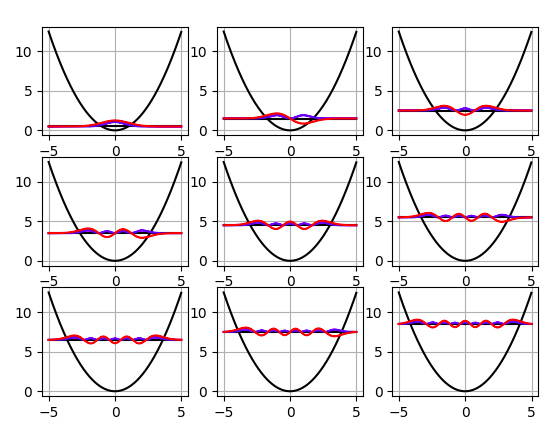
\includegraphics[width=0.4\textwidth]{images/harmonic_osc.png}}
\qquad
\subfloat[Step potential]{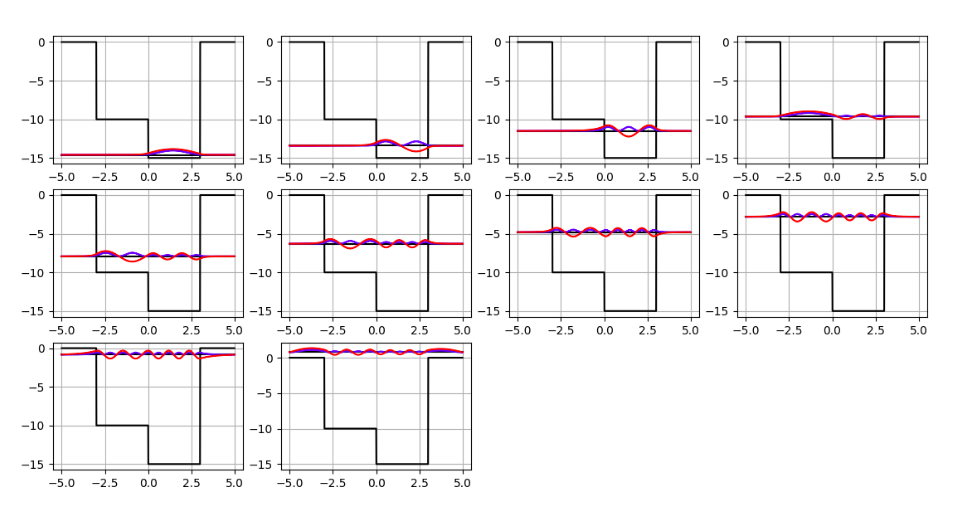
\includegraphics[width=0.5\textwidth]{images/potentialtise.png}}

\caption{Red curve is $\psi(x)$ and blue curve is $|\psi(x)|^2$}
\end{figure}


\newpage
\section{Transmittance and Reflectance using TISE}
Matching the value of the wavefunction and its derivative is done at the boundaries of the potential while finding the form of the wavefunction. By recasting this information in an appropriate way, we can construct a transfer matrix that gives us information on the reflectance and transmittance of a wave packet interacting with a potential. This arises from the fact that, the overall wave function can be thought of being decomposed into an "incoming" wave and an "outgoing" wave.
\\
\subsection{Single step potential}
Let us take a simple step potential, with values $V_1$ and $V_2$ on either side of the boundary, and let the wave function be $\psi(x)$
\\
\\
$$\psi(x) = A\psi_1(x) + B\psi_2(x)$$
$$\psi'(x) = A\psi_1'(x) + B\psi_2'(x)$$
\\
Writing it in matrix form;
\[
\begin{bmatrix}
\psi(x) \\
\psi'(x)
\end{bmatrix}
= \begin{bmatrix}
\psi_1(x) & \psi_2(x) \\
\psi_1'(x) & \psi_2'(x)
\end{bmatrix}
\begin{bmatrix}
A \\
B
\end{bmatrix}
\]
\\
Based on the values of E and V, the form of the wave function is oscillatory or exponential, and the matrix equation can be written as a product of simpler matrices, with the co efficients given by the table 1. (x is the boundary position and E is the energy of the particle)
\[
\begin{bmatrix}
\psi(x) \\
\psi'(x)
\end{bmatrix}
= K(V)E(V;x)
\begin{bmatrix}
A \\
B
\end{bmatrix}
\]

\begin{figure}[h!]
\center{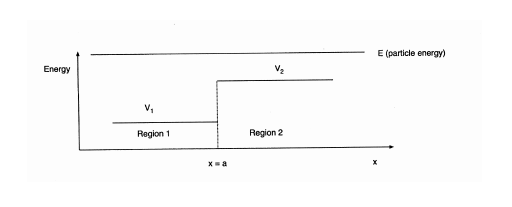
\includegraphics[width=0.6\textwidth]{images/1step.png}}
\caption{Single step potential configuration}
\end{figure}

Returning to the step potential, if the functions on either side of the boundary (x=a) are given as:

$\text{Region 1: } x\leq a$
$$\psi(x) = A\psi_1(x) + B\psi_2(x)$$

$\text{Region 2: } x > a$
$$\psi(x) = A\phi_1(x) + B\phi_2(x)$$

The continuity of the wavefunction and its derivative can now be written as:

\[
K(V_1)E(V_1;a)
\begin{bmatrix}
A \\
B
\end{bmatrix}
= 
K(V_2)E(V_2;a)
\begin{bmatrix}
C \\
D
\end{bmatrix}
\]

\[
\begin{bmatrix}
A \\
B
\end{bmatrix}
= 
E^{-1}(V_1;a)K^{-1}(V_1)K(V_2)E(V_2;a)
\begin{bmatrix}
C \\
D
\end{bmatrix}
\]

\begin{center}
\begin{table}
	\begin{tabular}{ |p{1.5cm}| p{5cm}  |p{4cm}|  p{5cm}|}
	\hline
	& $Case 1: E>V$ & Case 2: $E=V$& Case 3: $E<V$ \\
	& $k = \sqrt{2m(E-V)/\hbar^2}$ & & 	$k = \sqrt{2m(V-E)/\hbar^2}$ \\
	\hline	
	K(V) & 
	\[\begin{bmatrix}
	1 & 1 \\
	+ik & -ik 
	\end{bmatrix}\]
	 &
	\[\begin{bmatrix}
	1 & 0 \\
	0 & 1 
	\end{bmatrix}\]
	 &
	\[\begin{bmatrix}
	1 & 1 \\
	+k & -k 
	\end{bmatrix}\]
	\\
	
		$K^{-1}(V)$ & 
	\[\frac{1}{2}\begin{bmatrix}
	1 & \frac{1}{ik} \\
	1 & -\frac{1}{ik} 
	\end{bmatrix}\]
	 &
	\[\begin{bmatrix}
	1 & 0 \\
	0 & 1 
	\end{bmatrix}\]
	 &
	\[ \frac{1}{2}\begin{bmatrix}
	1 & -\frac{1}{k} \\
	1 & \frac{1}{k}
	\end{bmatrix}\]
	\\
	
		E(V;x) & 
	\[\begin{bmatrix}
	e^{ikx} &01 \\
	0 & e^{-ikx} 
	\end{bmatrix}\]
	 &
	\[\begin{bmatrix}
	1 & x \\
	0 & 1 
	\end{bmatrix}\]
	 &
	\[\begin{bmatrix}
	e^{-kx} & 0 \\
	0 & e^{kx} 
	\end{bmatrix}\]
	\\
	
		$E^{-1}(V;x)$ & 
	\[\begin{bmatrix}
	e^{-ikx} & 0 \\
	0 & e^{ikx} 
	\end{bmatrix}\]
	 &
	\[\begin{bmatrix}
	1 & -x \\
	0 & 1 
	\end{bmatrix}\]
	 &
	\[\begin{bmatrix}
	e^{kx} & 0 \\
	0 & e^{-kx} 
	\end{bmatrix}\]
	\\
	\hline
	\end{tabular}
	\caption{The matrices $K(V)$ and $E(V;x)$ and their inverses for the three cases.}
	\end{table}
\end{center}


\subsection{Piecewise constant potentials}
Any continuous potential can be broken down into small constant piecewise potentials, the previous section can be extended easily to this case to calculate the transfer matrix.
\begin{figure}[h!]
\center{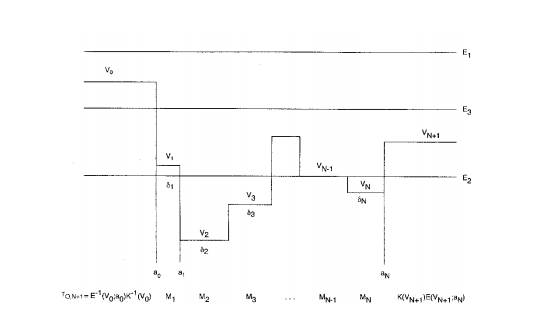
\includegraphics[width=0.6\textwidth]{images/steps.png}}
\caption{Combination of multiple step potentials}
\end{figure}

$$V(x) = V_j, \ a_{j-1} < x < a_{j}$$
\\
Let us take the solution in a region j to be;
$$\psi(x) = A_j\psi_1(x) + B_j\psi_2(x), \ a_{j-1} \leq x \leq a_j$$
\\
We can now relate the co efficients using the previous sections' results.

\[
\begin{bmatrix}
A_0 \\
B_0
\end{bmatrix}
= 
E^{-1}(V_0;a_0)K^{-1}(V_0)K(V_1)E(V_1;a_0)
\begin{bmatrix}
A_1 \\
B_1
\end{bmatrix}
\]

\[
\begin{bmatrix}
A_0 \\
B_0
\end{bmatrix}
= 
T_{01}
\begin{bmatrix}
A_1 \\
B_1
\end{bmatrix}
\]

\[
\begin{bmatrix}
A_1 \\
B_1
\end{bmatrix}
= 
T_{12}
\begin{bmatrix}
A_2 \\
B_2
\end{bmatrix}
\]
So we get the overall relation between co efficients to be: 
\[
\begin{bmatrix}
A_0 \\
B_0
\end{bmatrix}
= 
T_{01}T_{12}...T_{N-1,N}T_{N,N+1}
\begin{bmatrix}
A_{N+1} \\
B_{N+1}
\end{bmatrix}
\]

\[
\begin{bmatrix}
A_0 \\
B_0
\end{bmatrix}
= 
T_{0,N+1}
\begin{bmatrix}
A_{N+1} \\
B_{N+1}
\end{bmatrix}
\]

$$T_{j, j+1} = E^{-1}(V_j;a_j)K^{-1}(V_j)K(V_{j+1})E(V_{j+1};a_j)$$

For improving computational performance, the matrix can be broken down into a different way;
$$T_{j-1, j}T_{j,j+1} = E^{-1}(V_{j-1};a_{j-1})K^{-1}(V_{j-1}) \times \underbrace{K(V_j)E(V_j;a_{j-1})E^{-1}(V_j;a_j)K^{-1}(V_j)}_{M(V_j, \delta_j)}
\times K(V_{j+1})E(V_{j+1})E(V_{j+1}; a_j)$$

\begin{center}
\begin{table}
\centering
	\begin{tabular}{| p{5cm}  |p{3cm}|  p{5cm}|}
	\hline
	 $Case \ 1: E>V$ & $Case \  2: E=V$ & $Case \ 3: E<V$ \\
	 $k = \sqrt{2m(E-V)/\hbar^2}$ & & 	$k = \sqrt{2m(V-E)/\hbar^2}$ \\
	\hline	
	
	\[\begin{bmatrix}
	\cos(k\delta) & -k^{-1}\sin(k\delta) \\
	k\sin(k\delta) & \cos(k\delta) 
	\end{bmatrix}\]
	 &
	\[\begin{bmatrix}
	1 & -\delta \\
	0 & 1 
	\end{bmatrix}\]
	 &
	\[\begin{bmatrix}
	\cosh(k\delta) & -k^{-1}\sinh(k\delta) \\
	k\sinh(k\delta) & \cosh(k\delta) 
	\end{bmatrix}\] \\
	\hline
	\end{tabular}
	\caption{Real 2x2 matrices $M(V;\delta)$ for the three cases ($\delta_j = a_{j+1} - a_j$)}
	\end{table}
\end{center}
\subsection{Transfer matrix}
This algorithm will be used to compute the transfer matrices relating the amplitudes of the wavefunction at the leftmost region, $[A_L,B_L]^T$ and that of the rightmost region, $[A_R,B_R]^T$.

\[
E(V_L; a_0)
\begin{bmatrix}
A_L \\
B_L
\end{bmatrix}
= K^{-1}(V_L)M_1...M_NK(V_R)E(V_R;a_N)
\begin{bmatrix}
A_R \\
B_R
\end{bmatrix}
\]

\[
\begin{bmatrix}
A_L'\\
B_L'
\end{bmatrix}
= K^{-1}(V_L) \left \{\prod_{j=1}^N M(V_j;\delta_j) \right \} K(V_R) 
\begin{bmatrix}
A_R' \\
B_R'
\end{bmatrix}
\]

\[
M = 
\left \{\prod_{j=1}^N M(V_j;\delta_j) \right \}
=
\begin{bmatrix}
m_11(E) & m_{12}(E) \\
m_21(E) & m_{22}(E) 
\end{bmatrix}
\]

\[ 
T = \frac{1}{2}
\begin{bmatrix}
1 & \frac{1}{ik_L} \\
1 & \frac{-1}{ik_L}
\end{bmatrix}
%
\begin{bmatrix}
m_{11}(E) & m_{12}(E) \\
m_{21}(E) & m_{22}(E) 
\end{bmatrix}
%
\begin{bmatrix}
1 & 1 \\
ik_R & ik_R
\end{bmatrix}
\]

Computationally, we can calculate the M-matrix for every potential interval (except first and last) and multiply them using the above mentioned relation to find the transfer matrix. Using the elements of the T-matrix, we can then calculate the transmission/reflectance ratios.
\newpage
\subsection{Results}
By dividing any potential into piecewise step potentials, we can observe the transmittance ratio of the wave over any range of incident energy. Here are the transmission plots for a few potentials (inset graphs are the potential functions):
\begin{figure}[h!]
\centering
\subfloat[Transmission through Gaussian barrier]{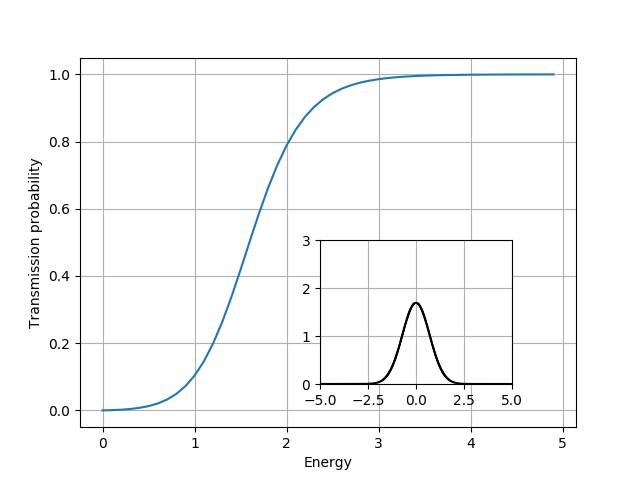
\includegraphics[width=0.4\textwidth]{images/gaussian_barrier.png}}
\qquad
\subfloat[Transmission through double well potential]{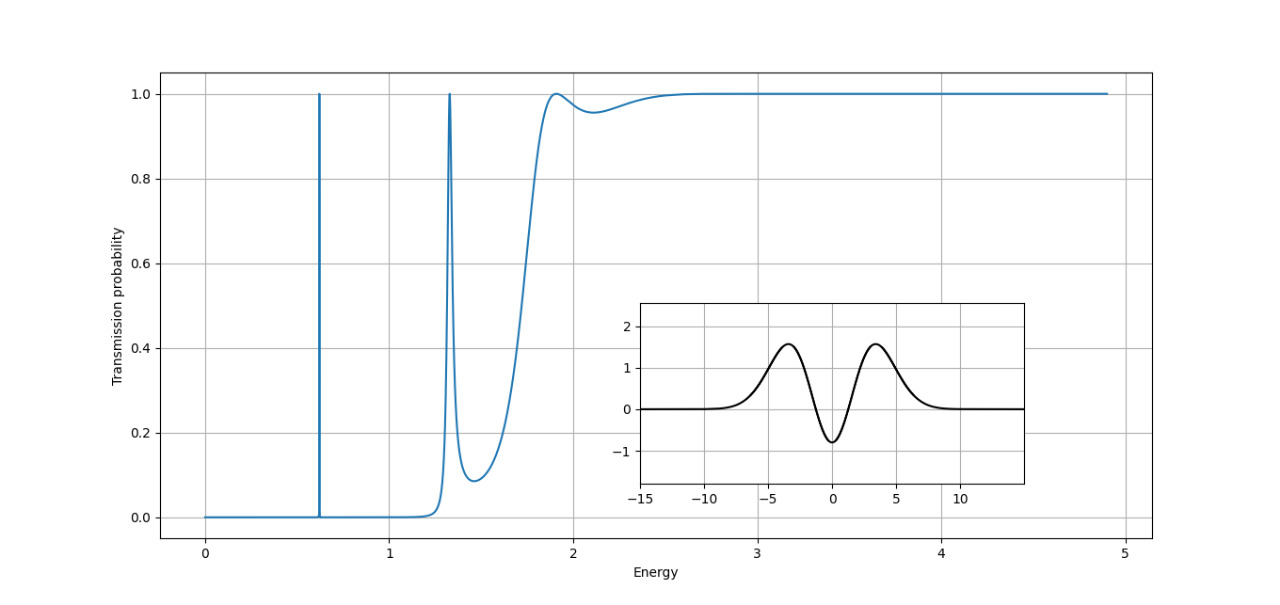
\includegraphics[width=0.5\textwidth]{images/double.jpeg}}

\end{figure}

\subsection{Observing emergence of resonance states in 1D well}
Resonance states are those wave functions having energy such that the transmission ratio through the potential is 1, i.e, perfect transmission. It can be observed that resonance states are closely connected to the bound states of the system. As we decrease the depth of the rectangular well, every time a bound state reaches threshold, a new resonance state is created.\cite{resonanceemergence}\cite{nussen}
\\
\\
The units used are $\hbar = m_e = 1$ (atomic units), so the energy is measured in the appropriate units. For this finite rectangular well of width 2.5$a_0$, as the depth is decreased from 7.5$E_h$ (bottom right plot), the fourth bound state threshold is at $\approx$ 6.9$E_h$, and we see a new resonance state appearing. Similarly, at E = 3.14$E_h$ (top right plot), which is the third bound state threshold, another resnonance state is formed. 
\begin{figure}[h!]
\center{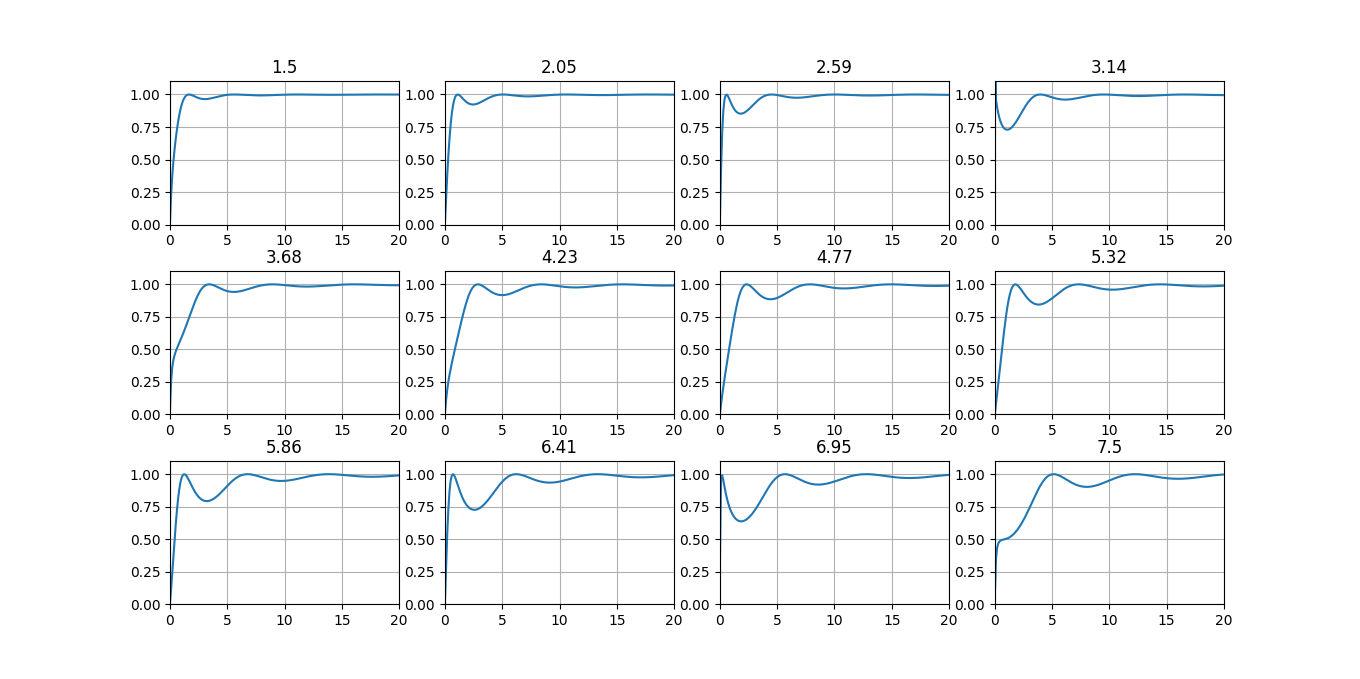
\includegraphics[width=\textwidth]{images/transmission_plot.png}}
\caption{Emergence of resonance states as well depth is decreased.}
\end{figure}


\newpage 
\section{Time Dependant Schrodinger Equation}
The time-dependant schrodinger equation in 1 dimension is given by:
$$i\hbar\frac{\partial}{\partial t} \psi(\textbf{x},t) = \hat{H}\psi(\textbf{x},t) ,\hspace{1 cm} \hat{H}=-\frac{\hbar^2}{2m}\frac{\partial^2}{\partial x^2} + V(\textbf{x},t)$$
To solve this numerically, we discretize the position grid x and the time t. 
$$x_n \rightarrow x_0+n\Delta x \hspace{1 cm} t_m = t_0+m\Delta t$$
If the potential is independant of time, the formal solution to the equation is given by: 
$$\psi(\textbf{x},\Delta t) = e^{-i\hat{H}\Delta t/ \hbar}\psi(\textbf{x},0) = \sum_{n=0}^{\infty} \frac{(-1)^n}{n!}\cdot\bigg( \frac{i\hat{H}\Delta t}{\hbar} \bigg )^n \psi(\textbf{x},0) = \hat{U}(\Delta t)\psi(\textbf{x},t)$$

where $\psi(\textbf{x},0)$ is the initial condition of the system, and $\hat{U}(\Delta t) = e^{-i\hat{H}\Delta t/\hbar}$ is the unitary propagation operator, and due to its unitarity, it preserves the inner product over time and the normalization of the wave function is maintained. The propagation operator is approximated here to simulate time evolution.

\subsection{Approximating the propagation operator}
One scheme to approximate the propagation operator is to cut off the taylor expansion from second degree terms (Euler method), however this requires small time steps for accuracy and the operator is no longer unitary.
$$\psi(\mathbf{x},t+\Delta t) = \bigg (1-\frac{i\Delta t}{\hbar}\hat{H} + \mathcal{O}(\Delta t)^2 \bigg ) \psi(\mathbf{x},t)$$

$$\bigg (1-\frac{i\Delta t}{\hbar}\hat{H} \bigg )\bigg (1-\frac{i\Delta t}{\hbar}\hat{H} \bigg )^\dagger = 1 + \frac{(\Delta t)^2}{\hbar^2} \hat{H}^2 \neq I$$

To preserve unitarity and avoid numerical instability, we can combine forward and backward euler methods in the following way.
\\
\\
\\
\subsection{Crank-Nicolson approximation}
Taking $\psi(x_n,t_m) \rightarrow \psi_n^m$, for convenience; 
$$\psi_n^{m+1} = [e^{-i\hat{H}\Delta t/\hbar}] \psi_n^m = [e^{-i\hat{H}\Delta t/(2\hbar)}\cdot e^{-i\hat{H}\Delta t/(2\hbar)}] \psi_n^m$$
$$[e^{i\hat{H}\Delta t/(2\hbar)}] \psi_n^{m+1} = [e^{-i\hat{H}\Delta t/(2\hbar)}] \psi_n^m$$
$$\bigg (1  +\frac{i\Delta t}{2\hbar}\hat{H} \bigg )\psi_n^{m+1} = \bigg (1-\frac{i\Delta t}{2\hbar}\hat{H} \bigg )\psi_n^m$$
Re-arranging this, we get the Crank Nicolson approximation, which is unitary and numerically stable.
$$\psi_n^{m+1} = \frac{\bigg (1-\frac{i\Delta t}{2\hbar}\hat{H} \bigg )}{\bigg (1+\frac{i\Delta t}{2\hbar}\hat{H} \bigg )} \psi_n^{m} + \mathcal{O}(\Delta t)^2$$

\newpage
Using finite differences to approximate the derivatives, we get:
$$\psi_m^{n+1} - \frac{i\Delta t}{2\hbar} \bigg[\frac{\hbar^2}{2m}\cdot \frac{\psi_{n+1}^{m+1} -2\psi_n^{m+1} +\psi_{n-1}^{m+1}}{(\Delta x)^2} - V_n\psi_n^{m+1} \bigg] =  \psi_m^{n} + \frac{i\Delta t}{2\hbar} \bigg[\frac{\hbar^2}{2m}\cdot \frac{\psi_{n+1}^{m} -2\psi_n^{m} +\psi_{n-1}^{m}}{(\Delta x)^2} - V_n\psi_n^{m} \bigg] $$

Setting $ \hspace{1 cm} \alpha = \frac{i\hbar \Delta t}{4m(\Delta x)^2} \hspace{1 cm} $, $\xi_n=\bigg[ 1 + \frac{i\Delta t}{2\hbar}\cdot (\frac{\hbar^2}{m(\Delta x)^2}+V_n)\bigg] \hspace{1cm}$, $\gamma_n=\bigg[ 1 - \frac{i\Delta t}{2\hbar}\cdot (\frac{\hbar^2}{m(\Delta x)^2}+V_n)\bigg]\\ \\ \\ \\ $ We now get a system of equations;

$$
(-\alpha)\psi_{n-1}^{m+1} + \xi_{n}\psi_n^{m+1} + (-\alpha)\psi_{n+1}^{m+1} = (\alpha)\psi_{n-1}^{m} + \gamma_{n}\psi_n^{m} + (\alpha)\psi_{n+1}^{m} \vspace{0.2cm}$$
Introducing $\pmb{\psi}^m = (\psi_0^{m}, ...,\psi_n^m, ...,\psi_N^m)$, we can recast it into a matrix equation; 
$$U_1\pmb{\psi}^{m+1} = U_2\pmb{\psi}^m$$
where, $U_1$ and $U_2$ are two (N+1) x (N+1) matrices.
$\\ \\  
\hspace{3cm} U_1=\begin{pmatrix}
    \xi_0 & -\alpha &           &      &  \\
  -\alpha & -\xi_1  & -\alpha   &      &   \\
          &  \ddots &  \ddots      & \ddots    &     \\
          &         &    -\alpha       &  \xi_{N-1}     & -\alpha \\
          &         &           &  -\alpha  & \xi_N
  \end{pmatrix}
$
$ \hspace{1cm}
U_2 =\begin{pmatrix}
     \gamma_0 & \alpha &         &             &  \\
      \alpha & \gamma_1& \alpha  &             &   \\
             &  \ddots &  \ddots & \ddots      &     \\
             &         & \alpha  & \gamma_{N-1}& \alpha \\
             &         &         &  \alpha     & \gamma_N
  \end{pmatrix}
$
\\
\\
\subsection{Algorithm}
\begin{algorithm}
\caption{2nd order Crank Nicolson approximation}
\begin{algorithmic}[1]

\Procedure{time_evolution}{$\mathbf{length}$}       
    \State Initialize $\mathbf{dx}$ and $\mathbf{dt}$ \Comment{grid resolution and time step}
    \State $\mathbf{xgrid}$ $\leftarrow$ list from $\mathbf{-length}$ to $\mathbf{+length}$ with $\mathbf{dx}$ spacing
    \State $\mathbf{M} \leftarrow$ number of time steps
    \State $\pmb{\psi_0} \leftarrow$ initial wavefunction  
    \State $\mathbf{V} \leftarrow$ list; potential configuration for each x in $\mathbf{xgrid}$
    \State
    \State Calculate lists $\pmb{\alpha}$, $\pmb{\xi}$, $\pmb{\gamma}$ according to given formula
    \State Initialize sparse tridiagonal matrices $\mathbf{U1, U2}$ using above lists
    \State Create empty complex matrix $\mathbf{PSI}$ of size N x M \Comment{N = length of xgrid}
    \State Assign $\mathbf{PSI}$[ ; ][0] = $\pmb{\psi_0}$
    \State Compute LU Decomposition of matrix $\mathbf{U1}$
    \State
    \For{m in range(0, M-2)}  
        \State Solve system U1*$\mathbf{PSI[\ ;\ ][m+1]}$ = U2*$\mathbf{PSI[\ ;\ ][m]}$ and compute $\mathbf{PSI[\ ;\ ][m+1]}$ 
        \State
        \State \Comment{PSI[ ; ][m] = (m)th column of PSI; value at $t=t_0+m\Delta t$}  
        \State 
    \EndFor
    \State Compute norm of each element of $\mathbf{PSI}$
    \State Return $\mathbf{normPSI}$
    \EndProcedure

\end{algorithmic}
\end{algorithm}
\subsection{Simulation}
The initial wave packet used to simulate an electron is a gaussian moving to the right;
$$\psi_0(x)=\frac{1}{\sqrt[4]{(\pi\sigma_0^2)}} \cdot exp\bigg[ ik_0 x - \frac{(x-\mu_0)^2}{2\sigma_0^2} \bigg]$$
A negative imaginary potential is used at either ends to prevent unwanted reflections.\cite{absorbV}

\begin{figure}[h!]
\center{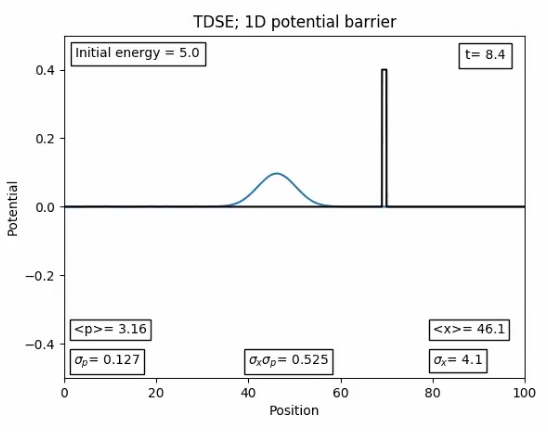
\includegraphics[width=0.5\textwidth]{images/gaussian.png}}
\caption{Gaussian wave packet}
\end{figure}


\subsection{Transmission through a double barrier}
The transmission ratio is obtained from the transfer matrix method using the TISE as discussed in the previous section. Using the TDSE simulation, after the wave packet impacts the potential barrier and disperses, the reflected and transmitted probability density is calculated to find the transmission ratio and is compared with the TDSE result.

\begin{figure}[h!]
\centering
\subfloat[Transmission ratios using TISE by calculating the transfer matrix]{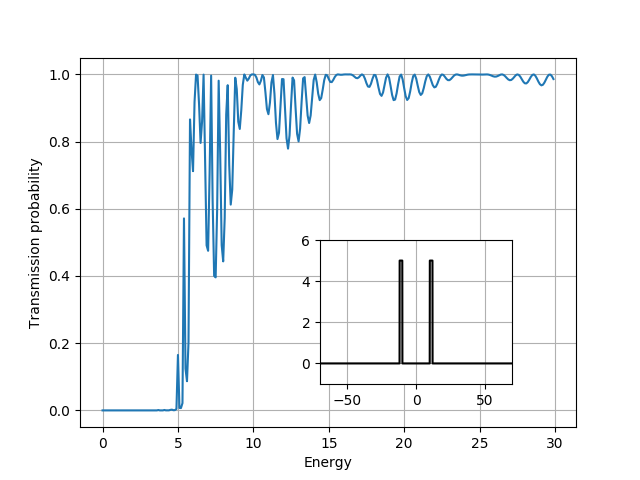
\includegraphics[width=0.4\textwidth]{images/doublewell_transmission.png}}
\qquad
\subfloat[Transmission ratios using TDSE for different values of spread in position of initial wave packet]{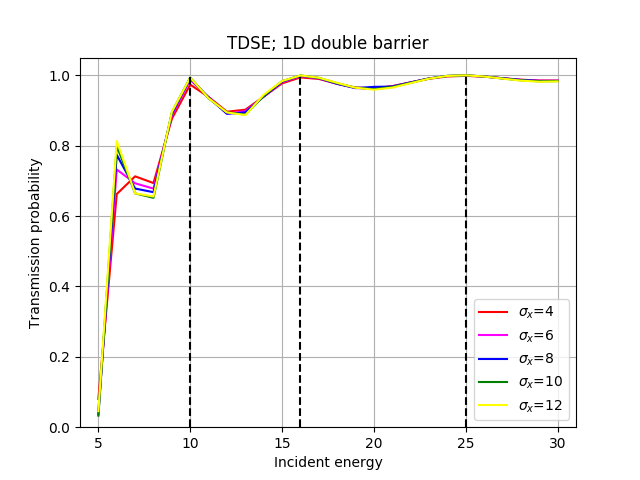
\includegraphics[width=0.4\textwidth]{images/finitewell_transmission2.png}}
\end{figure}

The energy levels of resonance states (100\% transmission) agree very well between the two, however the TDSE calculations seem to be an envelope of the TISE curve, but this might be due to the relatively bigger step size of energies taken to sample the ratios in the TDSE observations. Moreover, the initial uncertainty in position of the wave packet has been varied over a range but minimal deviation from the transmission ratios is observed which is a surprising result, as this directly relates to the spread of momenta and the uncertainty in the incident energy. 

\newpage

\section{TDSE with time varying potential}
The Crank Nicholson algorithm does not provide accurate results for time varying potentials, so here we use fourier transforms (as ffts are computed with ease) with the Split operator method. \cite{fft}

\subsection{Split operator method}

$$ i\hbar\frac{\partial \psi(r,t)}{\partial t} = \left [ -\frac{\hbar^2}{2m}\nabla^2 + V(r,t) \right ] \psi(r,t)$$

The split operator method is a pseudo-spectral differential equation solver. It relies on the fact that we can switch between position and momentum representations of the wavefunctions, and the position and momentum operators are multiplicative in their respective representations. So, we can split the hamiltonian into position space components, $\hat{H}_r = [V(r,t)]\psi(r,t)$ and momentum space components, $\hat{H}_k = \left [ -\frac{\hbar^2}{2m}\nabla^2 \right ] \psi(r,t)$. A general solution may be taken as:
$$\psi(r,t+dt) = \left [ e^{-\frac{i\hat{H}dt}{\hbar}} \right ] = \left [ e^{-\frac{i(\hat{H}_r + \hat{H}_k)dt}{\hbar}} \right ]$$
In order to have an error in the order of $dt^3$, we perform half step in position space, a full step in momentum space and the final half step in position space. This process is called Strang Splitting.
$$\psi(r,t+dt) = \left [ e^{-\frac{i\hat{H}_rdt}{2\hbar}}\cdot e^{-\frac{i\hat{H}_kdt}{\hbar}}\cdot e^{-\frac{i\hat{H}_rdt}{2\hbar}} \right ] + \mathcal{O}(t^3)$$

The straightforward algorithm then follows as performing a series of fast fouries transforms and multiplying by the respective values of position/momenta operators.

$$\psi(r,t+dt) = \left [ \hat{U}_r \left (\frac{dt}{2} \right ) \mathcal{F}^{-1}\left [ \hat{U}_k(dt)\mathcal{F}\left [\hat{U}_r \left (\frac{dt}{2} \right ) \psi(r,t) \right ] \right ] \right ] + \mathcal{O}(dt^3)$$
\\
This was used to simulate a wave packet incident on a fast oscillating single rectangular barrier potential, and attempts were made to locate conditions to attain 100\% transmittance but this was not achieved.

\section{Conclusion}
Several simple simulation methods were explored and observations on transmission of wave packets through potentials have been made. Other methods of using the numerov method (matching method to find energy values) have been attempted and implemented.
The split-op method was also extended to a 2D version to study the dynamics in a Henon-Heiles potential, but this was not done extensively. 

\begin{figure}[h!]
\centering
\subfloat[]{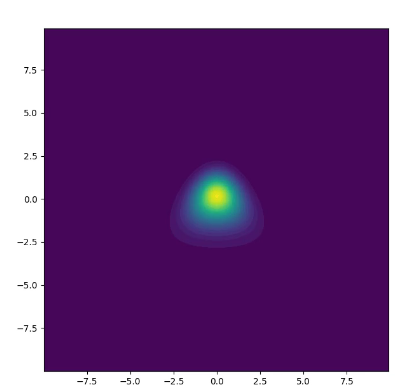
\includegraphics[width=0.3\textwidth]{images/henon2.png}}
\qquad
\subfloat[]{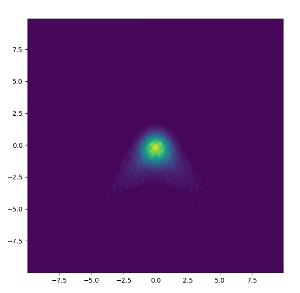
\includegraphics[width=0.285\textwidth]{images/henon.png}}
\caption{Attempt at 2D wave packet in henon-heiles potential}
\end{figure}

\newpage
\begin{thebibliography} {10}

\bibitem[1]{qmbook} Joshua Izaac, Jingbo Wang, 2019, Computational Quantum Mechanics

\bibitem[2]{tmatrix} Robert Gilmore, 2004, Elementary Quantum Mechanics in One Dimension

\bibitem[3]{resonanceemergence}  Raya Zavin and Nimrod Moiseyev 2004 J. Phys. A: Math. Gen. 37 4619

\bibitem[4]{nussen}  Nussenzveig H M 1959 Nucl. Phys. 11 499 

\bibitem[5]{absorbV} Nimrod Moiseyev 1998 J.Phys. B: Atomic. 31 1431

\bibitem[6]{fft} https://www.algorithm-archive.org/contents/split-operator_method/split-operator_method.html

 
\end{thebibliography}
\end{document}